\documentclass[twoside]{article}

\usepackage{epsfig}
\usepackage{amsmath}
\usepackage{booktabs}

\setlength{\oddsidemargin}{0.25 in}
\setlength{\evensidemargin}{-0.25 in}
\setlength{\topmargin}{-0.6 in}
\setlength{\textwidth}{6.5 in}
\setlength{\textheight}{8.5 in}
\setlength{\headsep}{0.75 in}
\setlength{\parindent}{0 in}
\setlength{\parskip}{0.1 in}

\newcommand{\lecture}[3]{
   \pagestyle{myheadings}
   \thispagestyle{plain}
   \newpage
   \setcounter{page}{1}
   \noindent
   \begin{center}
   \framebox{
      \vbox{\vspace{2mm}
    \hbox to 6.28in { {\bf CSE 291A/DSC 291:~Data Systems for Machine Learning, Spring 2026 \hfill} }
       \vspace{6mm}
       \hbox to 6.28in { {\Large \hfill #1  \hfill} }
       \vspace{6mm}
       \hbox to 6.28in { \it Lecturer: #2 \hfill 
        \parbox[t]{4.5in}{\raggedleft Scribes: #3} }
      \vspace{2mm}}
   }
   \end{center}
   \markboth{#1}{#1}
   \vspace*{4mm}
}

\begin{document}

\lecture{8: Runtime: Batching and Memory}{Hao Zhang}{Buwei Wu, Oren Nelson, Tzu Ping Chen, Tianyi Chen, \\Anyin Huang, Prabhleen Kaur, Ning Li, Yuheng Li}


\section{Big Picture: Where We Are}

In the previous lectures, we discussed several layers of deep learning systems. We first introduced the dataflow graph abstraction, where a machine learning program is represented as a graph of operators and tensors. We then discussed automatic differentiation, which allows the system to construct the backward pass from the forward computation. We also covered graph optimization, which is similar in spirit to traditional compiler optimization, except that the program being optimized is now a dataflow graph. In addition, we discussed operator optimization and compilation, where individual kernels such as matrix multiplication, convolution, and other tensor operators are implemented efficiently.

This lecture begins the discussion of \emph{runtime}. Once the graph has been built, differentiated, optimized, and lowered into executable operators, the system still has to run the graph efficiently. Runtime is where many practical systems problems appear. For example, even if every operator is individually optimized, the overall training job can still fail because the model, activations, or optimizer states do not fit in GPU memory. Similarly, a system may have enough total computation available, but poor scheduling or data movement can make the training loop slow.

At a high level, the topics in this runtime part include:
\begin{itemize}
    \item batching;
    \item checkpointing and rematerialization;
    \item swapping;
    \item quantization, mixed precision, and pruning.
\end{itemize}

These techniques are especially important for modern deep learning workloads because the models are often too large to fit comfortably on a single device. In this lecture, we start with the single-device or single-node setting. This is a simplified setting, but the ideas are still important because they are complementary to parallelization. Even when a model is distributed across many GPUs, each GPU still has limited memory, so runtime memory-saving techniques remain useful.

\section{Running the Graph with Minibatches}

After the graph is constructed and optimized, training repeatedly executes the graph over many batches of data. A typical training loop can be written as
\[
    \text{for } t = 1 \rightarrow N,
\]
where each iteration uses a batch of training data $D^{(t)}$ and updates the model parameters. Abstractly, the update can be written as
\[
    \theta^{(t+1)}
    =
    f\left(\theta^{(t)}, \nabla_{\theta} L\left(\theta^{(t)}, D^{(t)}\right)\right).
\]
Here, $\theta^{(t)}$ denotes the model parameters at iteration $t$, $D^{(t)}$ denotes the data batch used in that iteration, and $\nabla_{\theta} L$ denotes the gradient of the loss with respect to the parameters. The function $f$ represents the optimizer update rule. For example, for simple stochastic gradient descent, $f$ subtracts a learning-rate-scaled gradient from the current parameters. For more complex optimizers, such as Adam, $f$ also depends on additional optimizer states.

The important systems point is that each iteration is not just a mathematical update. It requires executing the forward pass, storing or recomputing intermediate values, executing the backward pass, and updating parameters. Therefore, runtime performance depends not only on floating point throughput, but also on memory capacity, memory lifetime, scheduling, and data movement.

\section{Why the Term ``Batch'' Is Ambiguous}

The word \emph{batch} is used in several different ways across machine learning, optimization, and data systems. Before discussing batching as a runtime technique, it is useful to separate these meanings.

In deep learning training, a batch usually refers to a group of training examples processed together. Instead of computing the gradient using the entire dataset, we sample a subset of examples and use this subset to estimate the gradient. This is the standard setting for stochastic gradient descent and its variants. In many practical contexts, people also use the terms \emph{batch} and \emph{mini-batch} interchangeably.

From the perspective of classical optimization, there is a distinction between full-batch gradient descent and stochastic gradient descent. In full-batch gradient descent, the entire dataset is used to compute one gradient update. This is usually impractical for deep learning because the full dataset is too large to fit in memory and too expensive to process at every step. In stochastic gradient descent, we instead use a smaller sampled batch. Under uniform sampling, the gradient computed from this smaller batch can be viewed as an unbiased estimate of the full-batch gradient. This is one reason stochastic gradient descent is widely used in machine learning.

In big data systems, the word batch has a different meaning. Batch processing usually means offline processing over a dataset that is already available. This is often contrasted with streaming or online processing, where data arrives over time and the system processes events as they arrive. Therefore, ``batch'' in big data systems refers more to the processing mode, while ``batch'' in deep learning usually refers to a group of training samples used in one or more training computations.

\section{Different Batch-Related Terms}

The following table summarizes the main meanings of several related terms.

\begin{center}
\begin{tabular}{lll}
\toprule
\textbf{Term} & \textbf{Context} & \textbf{Meaning} \\
\midrule
Batch & Deep learning & A group of training samples processed together \\
Mini-batch & Deep learning & A smaller subset of the dataset used for a training iteration \\
Micro-batch & Deep learning & A split of a mini-batch, often used for pipeline parallelism \\
Batch processing & Big data & Processing a large dataset in bulk/offline \\
Micro-batching & Big data & Processing small groups of events in short time windows \\
\bottomrule
\end{tabular}
\end{center}

The distinction between mini-batches and micro-batches becomes important later in the lecture. A mini-batch is the effective batch of data used for one parameter update, while a micro-batch is a smaller piece of that mini-batch. Micro-batches are useful when the full mini-batch does not fit in memory or when the system wants to improve hardware utilization. For example, in gradient accumulation, the system can process several micro-batches one by one, accumulate their gradients, and then apply one optimizer update. In pipeline parallelism, micro-batches help keep different pipeline stages busy at the same time.

\section{Memory Consumption}
Memory is one the most important concepts.  You cannot compute a workload if you are out of memory and you cannot compute it efficiently if you use the wrong kinds of memory.  The reason why the memory hierarchy exists is to speed up memory access and avoid memory bottlnecks. For a given workload to run, its peak memory must fit on available memory for the lifetime of the job. Available memory is defined as global memory such as High Bandwidth Memory (HBM) on GPU. Generally, there is no need to optimize peak memory as long as its less than available memory. 

$$ \max(\mathrm{memory}) < \mathrm{available\ memory} $$

There are three main sources of memory consumption in a model. (1) model weights, (2) activations (forward pass values), and (3) optimizer states (optimizers such as Adam etc.).


\section{Methods to Analyze Memory}
There are two main methods to analyze memory. (1) Size estimation i.e how many floating-point parameters are in the model. (2) For each floating-point parameter, how many bytes does it take up in memory.  For example, a model with 1 billion parameters and using 16-bit floating point precision would require roughly 2 GB of memory for the model weights alone.
% Please input person3's part Here

\section{Estimate size: Popular floating point standards}
For example, when we use FP32, we need 4 bytes to store per floating points and if we use FP16, we need 2 bytes instead.\\
FP16: Designed for general numerical computing. \\
BF16: It essentially "chops off" the fraction bits of a standard 32-bit float (FP32) while keeping the same exponent size.
\section{Estimate the weight size: GPT3}
What precision we use decides how many bits we need to store each parameters, and we almost always use FP16, so we usually get N*2. Batch size mwans how many tokens per batch.
\section{Estimate the activation size}
The parameter size is the number of elements we use multiply by 2 or 4(depends on the precision). bs means batch size, nc means number of channels. Activation size is bs*nc*wo*ho*(size of(element)).
\section{Estimate the activation size: MLP}
C=X*W , which is output=input*weight. The activation size is bs*m*p*sizeof(element), we only look at the output which is linear with bs since we need to store the activation per input example.
\section{Estimate the activation size:Transformers}
h means the embedding size for each word, and seq\_len indicates the number of tokens used per sequence. Here we can see that the input and ouput size are the same for transformer model.
% \section{Estimate the Activation Size}
\subsection{MLP}
We start with a fully connected layer, which is the basic building block of an MLP. Such a layer is essentially a matrix multiplication of the form: \[C = X W.\]

Suppose the input tensor $X$ has shape $\text{bs} \times m \times n$, where $\text{bs}$ is the batch size, $m$ is the number of input rows per example, and $n$ is the input feature dimension. The weight $W$ has shape $n \times p$. Then the output activation $C$ has shape $\text{bs} \times m \times p$, and its size in bytes is
\[
    \text{activation size}_{\text{matmul}}
    \;=\; \text{bs} \cdot m \cdot p \cdot \text{sizeof(element)}.
\]

\subsection{Transformers}

For a transformer layer, the activation tensor at the layer boundary typically has shape $\text{bs} \times h \times \text{seq\_len}$, where $h$ is the hidden dimension and $\text{seq\_len}$ is the sequence length. A transformer layer maps token representations to token representations, so its output has the same shape as its input. Treating the transformer layer as a black box, the per-layer activation size at the boundary is:
\[
    \text{activation size}_{\text{transformer}}
    \;=\; \text{bs} \cdot h \cdot \text{seq\_len} \cdot \text{sizeof(element)}.
\]

\subsubsection{A Numerical Example: GPT-3 Per-Layer Activations}

Considering one transformer layer of GPT-3, which has hidden dimension $d_{\text{model}} = 12288$, suppose the global token count for one iteration is $\text{bs} \cdot \text{seq\_len} \approx 3.2 \times 10^{6}$. The per-layer activation size is:
\[
    \text{bs} \cdot \text{seq\_len} \cdot d_{\text{model}}
    \;=\; 3.2 \times 10^{6} \cdot 12288
    \;\approx\; 3.93 \times 10^{10} \text{ elements}.
\]

Converting to bytes, using fp16 or bf16 ($2$ bytes per element), this is roughly $78$ GB per layer. Using fp32 ($4$ bytes per element), it doubles to roughly $156$ GB per layer.

These numbers are large for a single transformer layer. Importantly, this is only the boundary activation: each operator inside the layer also produces activations of its own, so the realistic per-layer cost is higher than the formula above suggests.

\section{Estimate the Optimizer State Size}
\subsection{Adam}
Adam is an adaptive optimizer that maintains running estimates of both the first and second moments of the gradient.

For each parameter, Adam keeps two additional tensors of the same shape as the parameter:
\begin{itemize}
    \item $m_t$: the first moment estimate, which is an exponential moving average of the gradient.
    \item $v_t$: the second moment estimate, which is an exponential moving average of the squared gradient.
\end{itemize}

Both $m_t$ and $v_t$ are updated at every step and are required to compute the next parameter update. Because they share the parameter shape, their memory cost scales linearly with the number of parameters.

\subsection{Total Adam State Cost}

Putting these pieces together, the per-step optimizer-related memory for Adam consists of three components, each of size $N \cdot \text{sizeof(element)}$, where $N$ is the total number of parameters:
\begin{itemize}
    \item $\nabla_{\theta} L$: the gradient with respect to parameters;
    \item $m_t$ the first moment estimate;
    \item $v_t$ the second moment estimate.
\end{itemize}

The total optimizer-related memory cost is therefore:
\[
    \text{optimizer memory}
    \;=\; 3 N \cdot \text{sizeof(element)}.
\]

% Scribe section by Anyin Huang
% Slides covered: pages 22--26

\section{Memory Overview}
Taking GPT-3 (175B parameters) as an example, the memory cost of model parameters is about 350 GB (FP16) or 700 GB (FP32). 
The activations, estimated only at transformer layer boundaries for 96 layers, consume about 7488 GB (FP16) or 14976 GB (FP32), though actual internal activations would be higher. 
The optimizer states consume about 12 * 175 GB (FP32) of memory.

\section{Reduce Activation Memory}
In standard training, we store all intermediate activations to compute gradients during the backward pass, leading to an O(N) memory cost for an N-layer network. 
Activation Checkpointing aims to reduce this peak memory by exploiting the fact that activations are not needed until the backward pass. 
Option one is dicard nothing. 
Option two is dicard all and recompute for each layer.
We want to strike a balance. 
The idea is that the activation is not needed again until the backward pass comes, discard some of them and recompute the missing intermediate nodes in small segments. 
For an N-layer neural network, if we place a checkpoint every K layers, the total activation memory cost can be modeled as: Memory Cost = O(N/K) (Checkpoint cost) + O(K) (Re-computation cost). 
By minimizing the cost function, we find the optimal solution at K= $\sqrt{N}$.
\section{Discussion of Gradient Checkpointing}
The below image provides a visual illustration of what the memory lifetime looks like with and without checkpointing. With rematerializing activations the blue curve shows that we use way lesser RAM than if we retain all activations as in the red curve. 
Gradient Checkpointing is also called rematerialization or recomputation. In practice, you can activate gradient recomputation in PyTorch using torch.utils.checkpoint API.

\begin{figure}[h]          % h=here, t=top, b=bottom, p=page
    \centering
    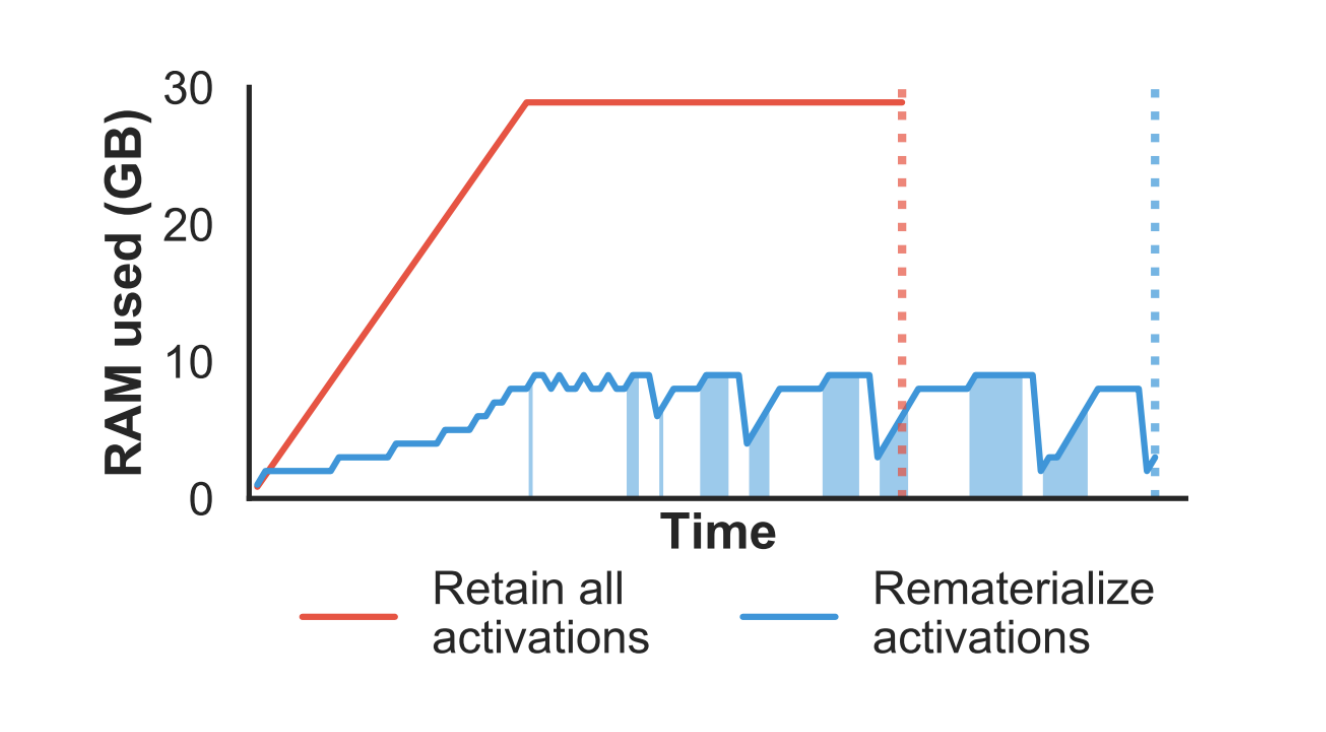
\includegraphics[width=0.8\textwidth]{memory_dynamics.png}
    \caption{Memory Dynamics}
    \label{fig:memory_dynamics}    % for cross-referencing
\end{figure}
Cons of this approach are that this only helps with the activation memory, not with weight or optimizer memory. If we have plenty of memory, we can retain all activations and we don't have to spend extra time recomputing them.

When thinking about the optimal checkpointing policy we need to consider things like the memory of the layers to be checkpointed (since different layer out's have different sizes) and the recomputation cost of the non-checkpointed layers since it won't be the same for all layers

\section{Similar approach: Gradient Accumulation}
Rematerialization wastes some compute by design. Gradient accumulation prevents that by keeping a small buffer of accumulated gradients. When the hardware can't fit your desired batch size, you run the training loop with smaller microbatches and accumulate the gradients into the buffer. We run iterations of microbatches and fill the buffer till desired batch size is reached and then run the gradient update.
However with this approach, in some cases when microbatches are too small, we risk having very low Arithmetic Intensity and poor GPU utilization. 
% Scribe section by Ning Li
% Slides covered: pages 32--36


\section{Move to DRAM}

Gradient checkpointing and gradient accumulation only help with activation memory. They do not reduce the memory used by weights or optimizer states. To handle those, we use a different idea.

A typical training server actually has plenty of memory. It is just not on the GPU. For example, a machine with H100 or H200 GPUs usually has around one terabyte of CPU DRAM, while each GPU only has 40 to 80 GB of HBM. So if a tensor does not fit in HBM, we can try to put it in DRAM instead. The problem is that DRAM is much slower than HBM, and the GPU cannot read from it directly. The relevant numbers are summarized below. To solve such problem, we introduce the CPU SwapIn and SwapOut.

\begin{center}
\begin{tabular}{lll}
\toprule
\textbf{Tier} & \textbf{Bandwidth} & \textbf{Capacity} \\
\midrule
GPU SRAM & 19 TB/s   & 20 MB \\
GPU HBM  & 1.5 TB/s  & 40 GB \\
CPU DRAM & 12.8 GB/s & $>$1 TB \\
\bottomrule
\end{tabular}
\end{center}

\subsection{CPU Swap}

To use DRAM as extra memory, we introduce two new operations:
\begin{itemize}
    \item \texttt{SwapOut}: copy a tensor from HBM to CPU DRAM.
    \item \texttt{SwapIn}: copy a tensor from CPU DRAM back to HBM.
\end{itemize}
This is called CPU swapping. Unlike checkpointing or accumulation, it applies to both weights and activations.

The reason swapping works is that, at any given moment, the GPU is only computing on one operator. Tensors from operators that have already finished, or operators that have not started yet, do not need to stay in HBM. So during the forward pass, we can swap out tensors that have just been used. During the backward pass, we swap them back in before they are needed again. Swapping is a scheduling problem, so the runtime can run \texttt{SwapIn} on a separate stream and overlap it with the computation of an earlier layer. If the prefetch finishes in time, the swap is essentially free.

\subsection{When Does Swapping Work?}

Whether swapping is actually free depends on a simple comparison. The time to swap a tensor is
\[
T_{\text{swap}} \;=\; \frac{\text{tensor size}}{\text{bandwidth}}.
\]
For the prefetch to be hidden, we need $T_{\text{swap}} \le T_{\text{compute}}$, where $T_{\text{compute}}$ is the time the GPU spends on the layers in between.

This condition is hard to satisfy on modern GPUs. Compute throughput on Blackwell-class hardware has grown much faster than memory bandwidth. So the GPU often finishes its current work before the next prefetch arrives, and then it has to wait. In practice, academic groups with limited GPU budgets still use swapping because they have no choice. Large industry labs usually avoid it because it makes training too slow.

\section{Summary of Memory Optimizations}

We have now seen three single-device techniques to fit a workload into limited GPU memory:
\begin{itemize}
    \item \textbf{Gradient checkpointing}: trade compute for memory. Only applies to activations.
    \item \textbf{Gradient accumulation}: reduce the effective micro-batch size while keeping the same total batch size for each update.
    \item \textbf{CPU swapping}: use a lower tier of the memory hierarchy. Applies to both weights and activations.
\end{itemize}

One thing to notice is that none of these techniques actually changes the size of any tensor. The shapes of weights, activations, and optimizer states all stay the same. What they change is the \emph{lifetime} of each tensor, that is, when it has to be on the GPU. So all three are scheduling techniques. They reshape the memory dynamics so that the peak HBM usage stays below the device capacity. The other direction is to reduce the original size itself, for example by using lower precision such as FP16, FP8, or FP4. This is the topic of the next lecture.

\section{In-Class Questions}

\subsection{Sources of Memory Consumption}

\textbf{Q: Which of the following is \emph{not} one of the main sources of memory consumption?}
\begin{itemize}
    \item[A.] Intermediate activation values
    \item[B.] Model weights
    \item[C.] Optimizer states
    \item[D.] Training code
\end{itemize}

The answer is \textbf{D}. The three main sources are weights, activations, and optimizer states. For example, the training code of GPT-3 is only a few kilobytes, so it is negligible.
% Scribe section by Yuheng Li
% Slides covered: pages 37 -- 39

\subsection{Properties of Gradient Checkpointing}

\textbf{Q: Which of the following statements is \emph{false} about gradient checkpointing?}
\begin{itemize}
    \item[A.] Applying gradient checkpointing during model training could save GPU memory.
    \item[B.] Gradient checkpointing applies to both model weights and activations.
    \item[C.] The location of gradient checkpointing affects how much re-computation and memory are needed.
    \item[D.] It is possible to discard some of the activations from memory since they are only needed during the backward pass.
\end{itemize}

The answer is \textbf{B}. Gradient checkpointing is fundamentally a technique for activation memory only. It works by discarding intermediate activations after the forward pass and recomputing them on demand during the backward pass. Model weights, by contrast, must remain both the forward and the backward computation, as there is no possible way to recompute them during the backward pass, so the same trick cannot be applied to them.

\subsection{Activation Size of GPT-3 2.7B}

\textbf{Q: Given the table of GPT-3 model configurations, what is the activation size of GPT-3 2.7B (using fp16 for all activations and checkpointing at the transformer layer boundary)?}
\begin{itemize}
    \item[A.] $7031.25$ GB
    \item[B.] $201.34$ GB
    \item[C.] $152.59$ GB
    \item[D.] $305.18$ GB
\end{itemize}

The answer is \textbf{C}. The relevant entries from the configuration table for GPT-3 2.7B are:
\begin{center}
\begin{tabular}{lr}
\toprule
$n_{\text{layers}}$ & $32$ \\
$d_{\text{model}}$ & $2560$ \\
Batch size (tokens per step) & $1\text{M} = 10^6$ \\
\bottomrule
\end{tabular}
\end{center}

When we checkpoint at the transformer layer boundary, the only activation we keep on device per layer is the input to that layer, whose shape is $(B \cdot S) \times d_{\text{model}}$, where $B \cdot S$ is the total number of tokens in the batch. The size of one such checkpoint, in bytes, is
\[
\underbrace{(B \cdot S)}_{10^6} \;\times\; \underbrace{d_{\text{model}}}_{2560} \;\times\; \underbrace{2}_{\text{fp16}} \;=\; 5.12 \times 10^9 \text{ bytes}.
\]
We keep one such checkpoint per layer, and there are $n_{\text{layers}} = 32$ layers, so the total activation memory is
\[
32 \;\times\; 5.12 \times 10^9 \;=\; 1.6384 \times 10^{11} \text{ bytes}.
\]
Converting to gibibytes ($1\text{ GiB} = 2^{30}$ bytes),
\[
\frac{1.6384 \times 10^{11}}{2^{30}} \;\approx\; 152.59 \text{ GiB}.
\]

\section{How to Choose/Tune Memory Optimization}

We now have three memory-saving techniques for a single device: gradient accumulation, gradient checkpointing, and CPU swapping. In practice, these methods are often used together, and usually in that order, from the least expensive to the most expensive in terms of training speed. The goal is to fit the workload on one device while still keeping the job completion time (JCT) acceptable.

\begin{enumerate}
    \item \textbf{Choose the target global batch size} (for example, $64$). This is usually set by the training setup and should stay fixed. The methods below do not change the effective batch size; they only change how that batch is run.

    \item \textbf{Try training with that batch size directly.} If the job runs without an OOM, then no memory optimization is needed.

    \item \textbf{If OOM happens, first use gradient accumulation.} Reduce the micro-batch size step by step ($32 \to 16 \to 8 \to \ldots$) while keeping the global batch size fixed. This is usually the cheapest option, since it does not add much extra computation. It only splits the same batch into more smaller steps before each parameter update.

    \item \textbf{If gradient accumulation is still not enough, add gradient checkpointing.} Use the largest micro-batch size that fits in HBM, and recompute some activations during backpropagation instead of storing them all. This saves more memory, but it slows training down more than gradient accumulation.

    \item \textbf{If the model still does not fit, turn on CPU swapping.} This is usually the most expensive option, because data must move between GPU memory and CPU memory, and CPU memory bandwidth is much lower than HBM bandwidth.

    \item \textbf{Check whether the JCT is still acceptable.} All of these methods make training slower to some degree. If the final JCT is still within budget, then the setup is good. If not, the single device setup is no longer enough, and the next step is to use multiple devices, i.e., parallelism.
\end{enumerate}

The main idea is simple: always try the option with the smallest slowdown first, and only move to a heavier method if needed. Also note that these methods do not change tensor shapes. They mainly change when a tensor needs to stay on the GPU, not how large the tensor is. Reducing tensor size itself, for example, by using lower precision such as FP8, or FP4, is a separate topic(Quantization).

\end{document}